\section{Architettura del sistema}
L'applicazione ADCrm presenta un'architettura client-server, assumendo entrambi i ruoli:
\paragraph{Server}
L'applicazione assume il ruolo di server nel momento in cui deve assolvere alle richieste che arrivano da ADProject mediante le API REST. Deve quindi rispondere ad un'esigenza principale due esigenze:
\begin{itemize}
	\item esporre API REST per poter rispondere, in formato \glo{JSON}, alle richieste HTTP ricevute;
	\item salvare le credenziali per il processo di autenticazione e collegamento con il CRM su un piccolo database interno.
\end{itemize} 

Si è deciso di mantenere il database sul servizio ADCrm per togliere l'onere ad ADProject di conoscere: non solo le procedure di autenticazione al CRM, ma anche la tipologia di CRM che si va ad interrogare (Salesforce, Dynamics, ...). In questo modo si riesce a mantenere una netta separazione dei ruoli tra le varie componenti. 

\paragraph{Client}
L'applicazione funge da client nel momento in cui deve interrogare il server del CRM per recuperare i dati di cui ha bisogno ADProject; deve quindi:
\begin{itemize}
	\item interrogare il server remoto attraverso il set di API che espone;
	\item organizzare i dati ricevuti in modo tale che siano fruibili da ADProject.
\end{itemize}

Nelle prime fasi della progettazione si è valutata l'ipotesi di utilizzare un database per fare \glo{caching} dei dati provenienti dal CRM, così da limitare le richieste HTTP necessarie e da velocizzare le risposte fornite, tuttavia la necessità di ADProject di utilizzare sempre dati aggiornati ha fatto abbandonare quest'opzione.\\

La figura \ref{fig:architetturasistema} illustra l'architettura ad alto livello del sistema; una descrizione più dettagliata delle varie componenti verrà esposta nelle sezioni successive.

\begin{figure}[H]
	\centering
	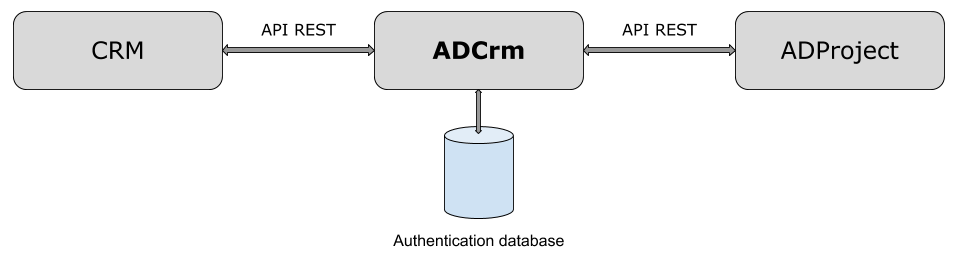
\includegraphics[width=\linewidth]{images/architettura_sistema}
	\caption{Architettura ad alto livello}
	\label{fig:architetturasistema}
\end{figure}

\section{API REST}\label{apiRest}
Di seguito si trova la definizione delle API REST esposte dal servizio ADCrm.\\
I metodi HTTP con cui chiamare tutti i successivi URL sono metodi \textbf{GET} ed i dati ricevuti nelle risposte sono forniti in formato \glo{JSON}.

	\begin{small}
		\begin{longtable}{ | l | p{8cm} | }
			\hline \textbf{URL} & \textbf{Descrizione Risposta}\\
			\hline api/organization/\{organizationId\}/ & Risponde con i dati riguardante l'organizzazione avente \textit{id = organizationId}\\
			\hline
		\end{longtable}		
	\end{small}
Questo primo \glo{endpoint} necessita di ulteriori spiegazioni in quanto l'url specificato sopra è da anteporre a di tutti quelli che seguiranno (eg. "\textbf{api/organization/\{organizationId\}/accounts}" nel caso dell'url "/accounts").\\
Inoltre si noti che è necessario da parte di chi effettua chiamate verso questo url (e quindi anche verso tutti gli altri) conoscere il campo \textit{organizationId} per poter ottenere una risposta. Questa restrizione è stata posta per far si che il sistema sia più sicuro, rendendo disponibili dei dati riguardanti l'azienda fruitrice del servizio solo se si conosce il corretto identificativo.
%TODO: decidere se sistemare la parte qua sopra
	\begin{small}
		\begin{longtable}{ | l | p{8cm} | }
			\hline \textbf{URL} & \textbf{Descrizione Risposta}\\
			\hline /accounts & Risponde con la lista contenente i dati di tutti gli account\\
			\hline /accounts/\{\textit{accountId}\} & Risponde con i dati dell'account avente \textit{id = accountId}\\    
			\hline /accounts/\{\textit{accountId}\}/contacts & Risponde con la lista contenente i dati di tutti gli i contatti legati all'account avente \textit{id = accountId}\\
			\hline /accounts/\{\textit{accountId}\}/proposals & Risponde con la lista contenente i dati di tutte le offerte commerciali legate all'account avente \textit{id = accountId}\\
			\hline /contacts/\{\textit{contactId}\} & Risponde con i dati del contatto avente \textit{id = contactId}\\
			\hline /proposals & Risponde con la lista contenente i dati di tutte le proposte commerciali\\
			\hline /proposals/\{\textit{proposalId}\} & Risponde con i dati della proposta commerciale avente \textit{id = proposalId}\\    
			\hline /proposals/\{\textit{proposalId}\}/products & Risponde con una lista contenente tutti i prodotti legati all'offerta commerciale avente \textit{id =  proposalId}\\
			\hline /products/\{\textit{productId}\} & Risponde con i dati del prodotto avente \textit{id = productId}\\
			\hline /users & Risponde con una lista contenente i dati di tutti gli utenti del CRM\\
			\hline /users/\{\textit{userId}\} & Risponde con i dati del utente avente \textit{id = userId}\\    
			\hline /productCategories & Risponde con una lista contenente i dati di tutte le famiglie di prodotti\\
			\hline /productCategories/\{\textit{categoryId}\} & Risponde con i dati della famiglia di prodotti avente \textit{id = categoryId}\\		
			\hline 
		\end{longtable}		
	\end{small}
	
\section{Progettazione di dettaglio}

\begin{figure}[H]
	\centering
	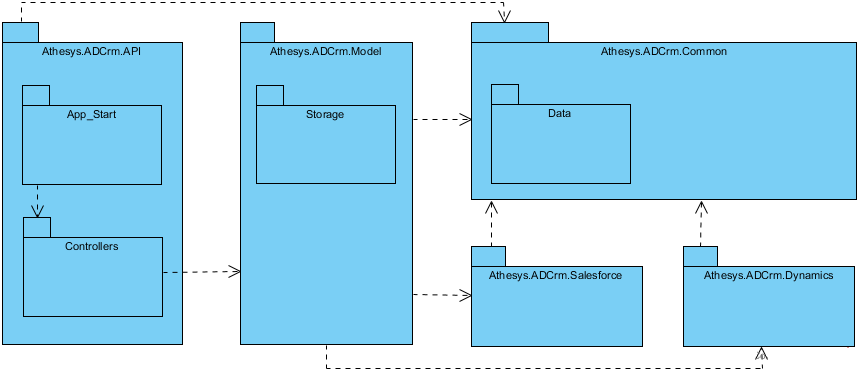
\includegraphics[width=\linewidth]{images/modulesDiagram}
	\caption{Diagramma dei moduli di ADCrm}
	\label{fig:generalUMLDiagram}
\end{figure}

\begin{figure}[H]
	\centering
	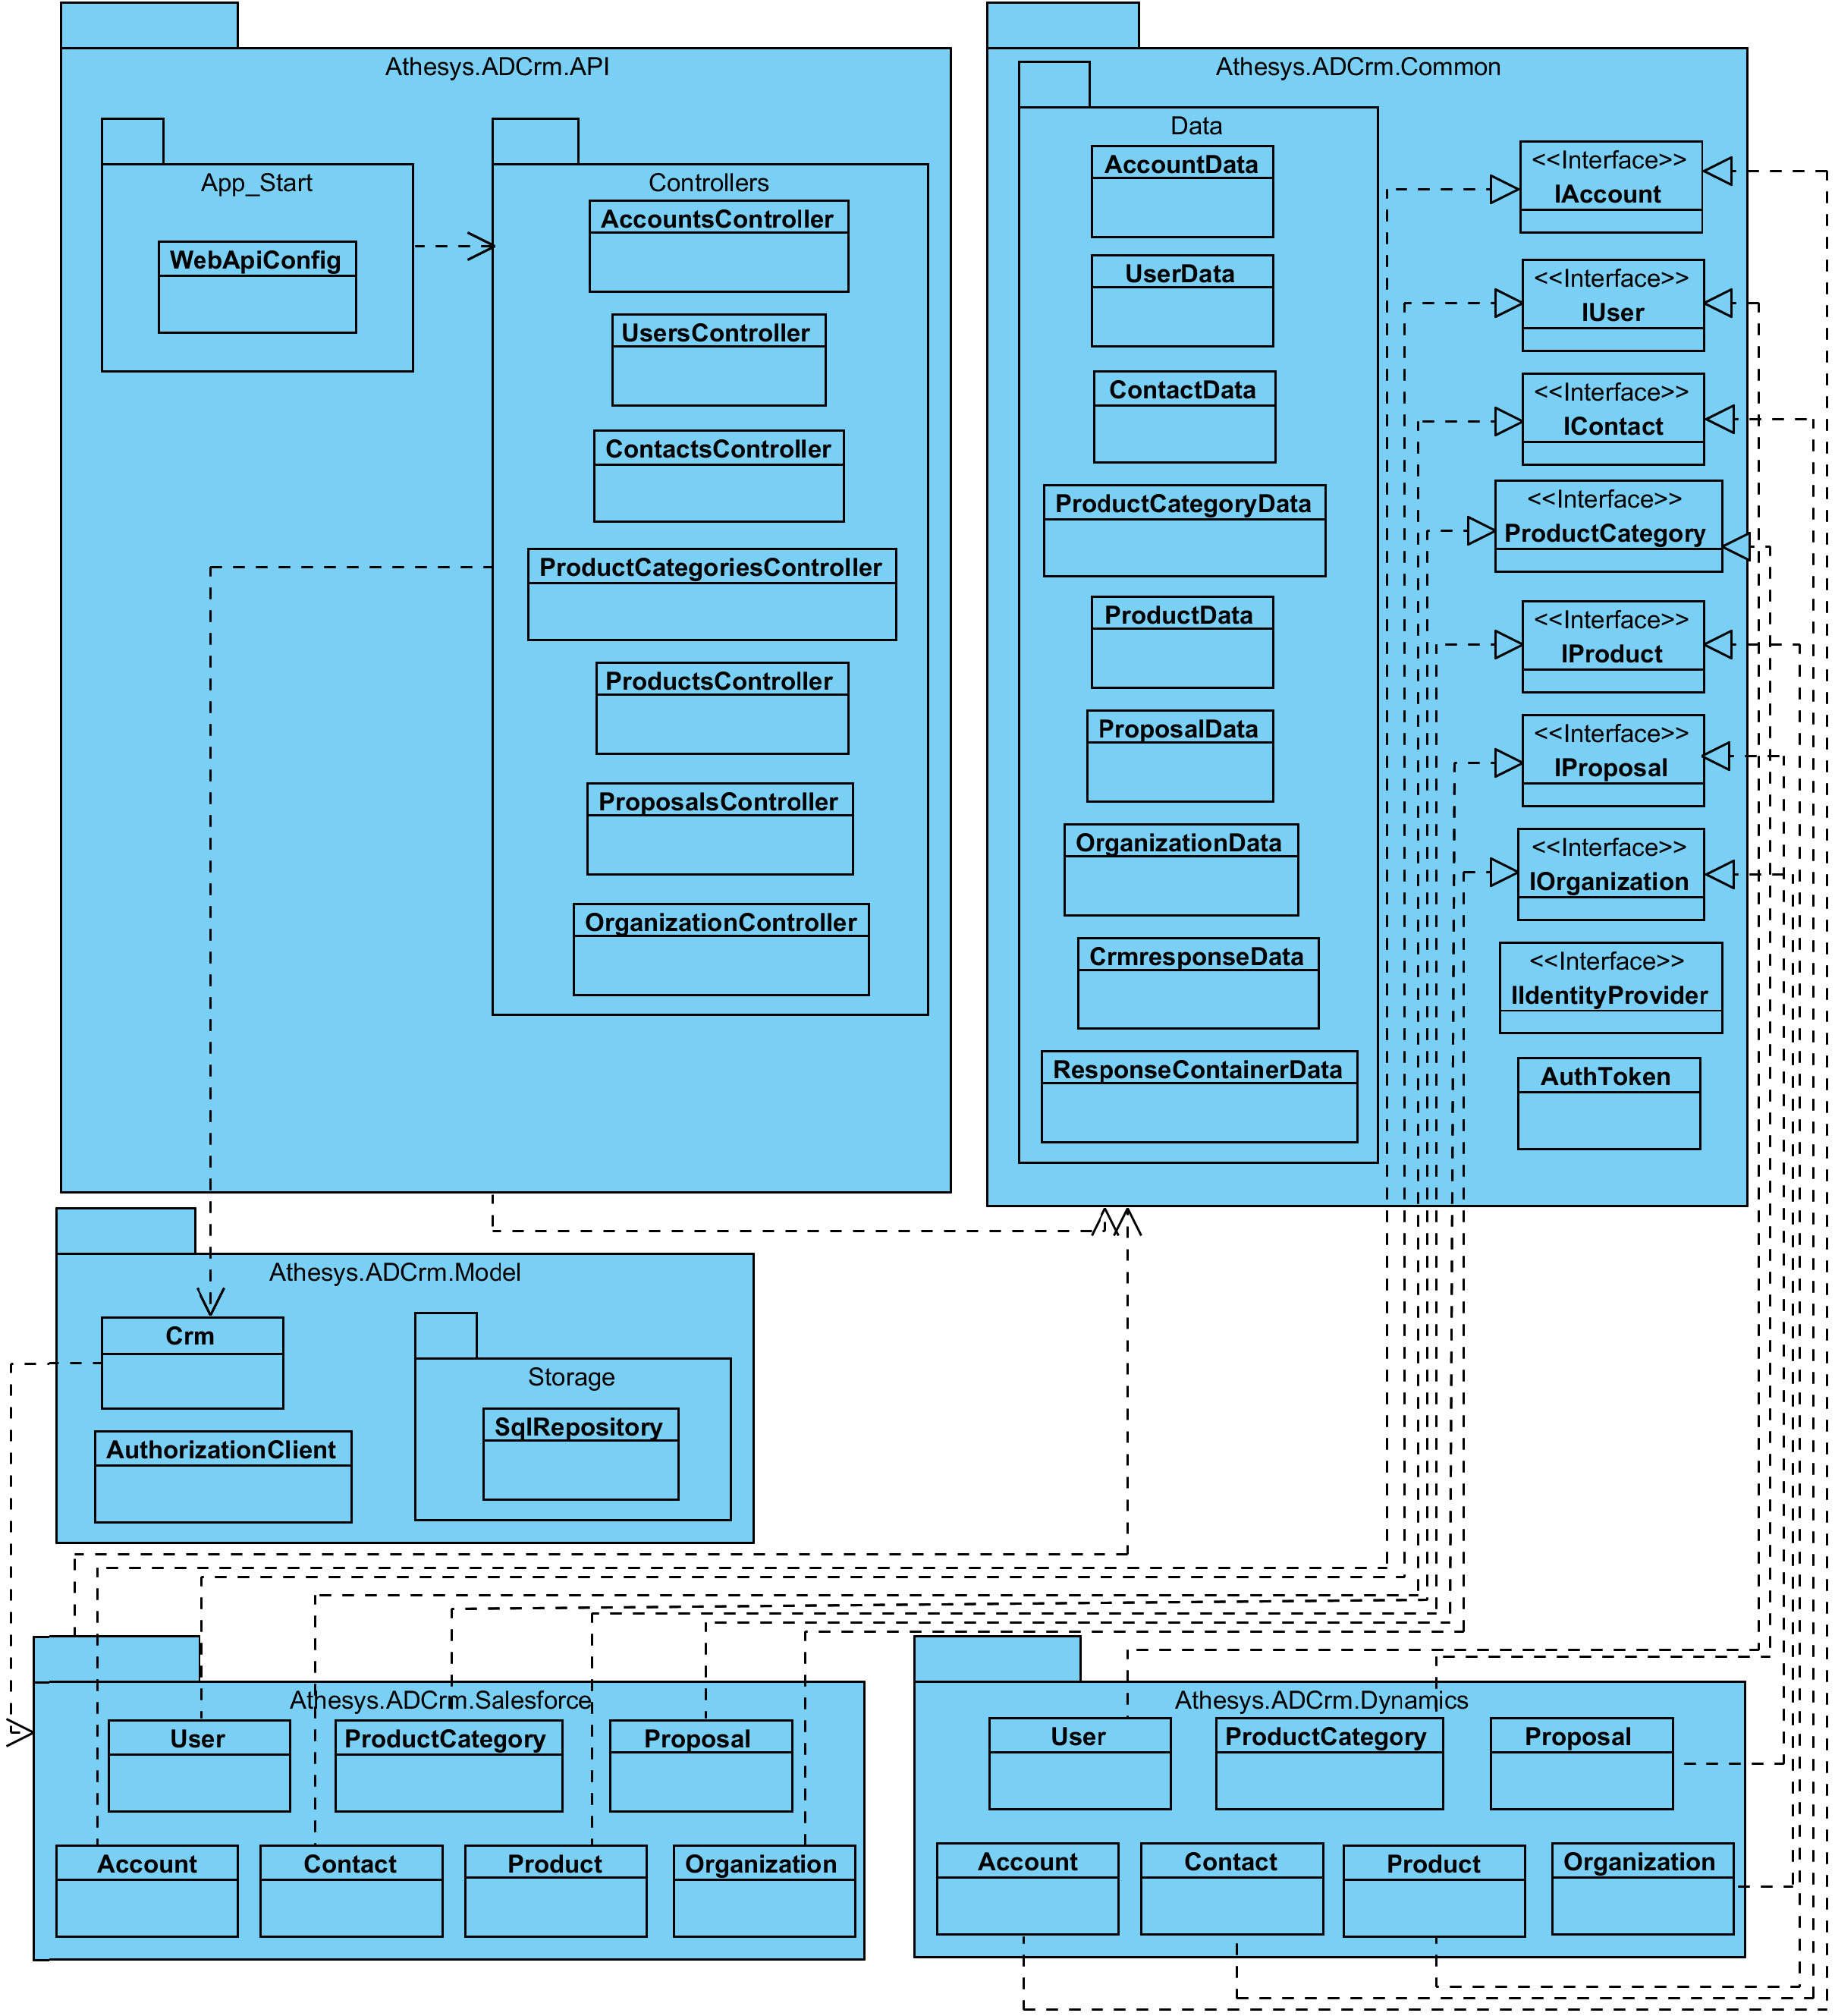
\includegraphics[width=\linewidth]{images/general2}
	\caption{Diagramma UML di ADCrm}
	\label{fig:modulesdiagram}
\end{figure}



\subsection{Athesys.ADCrm.API}

\begin{figure}[H]
	\centering
	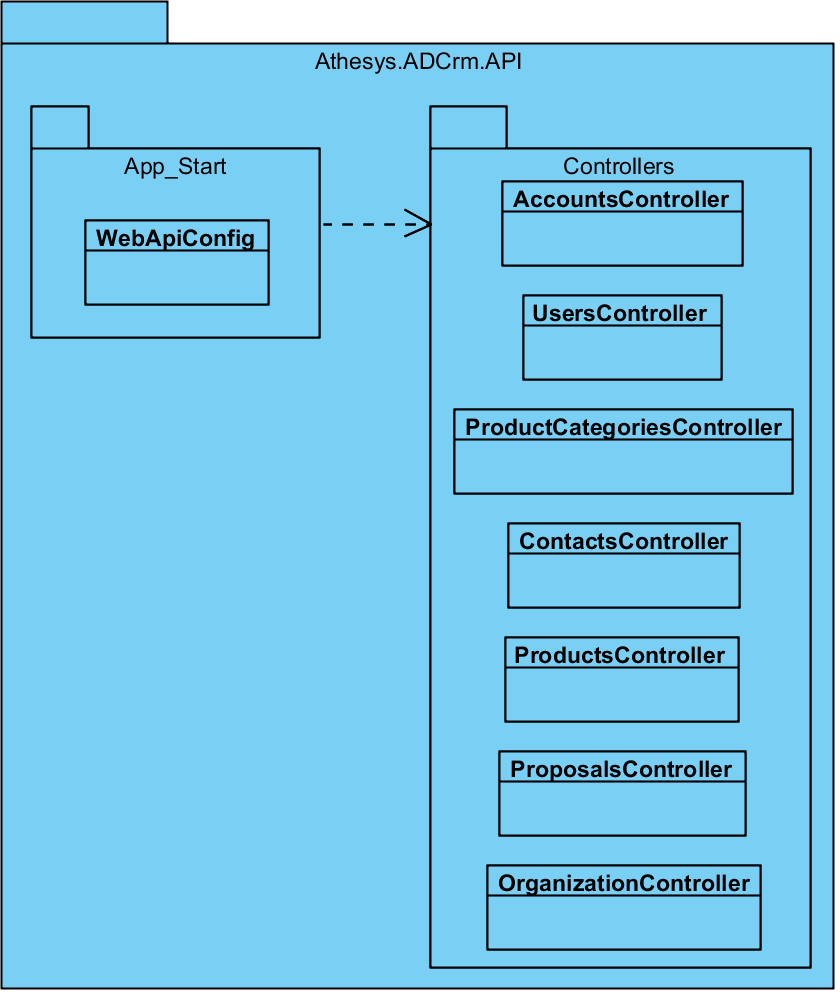
\includegraphics[width=\linewidth]{images/modules/API}
	\caption{}
	\label{fig:api}
\end{figure}

Questo \glo{package} è utilizzato per esporre le API REST all'applicazione web ADProject. In esso vengono definite le \glo{route} che è possibile chiamare e ad ognuna di esse viene associato un metodo di un particolare controller. 

\subsection{Athesys.ADCrm.API.AppStart}
Questo \glo{package} contiene la classe che si occupa di definire le \glo{route} che verranno esposte dall'applicazione.

\subsection{Athesys.ADCrm.API.Controllers}

\begin{figure}[H]
	\centering
	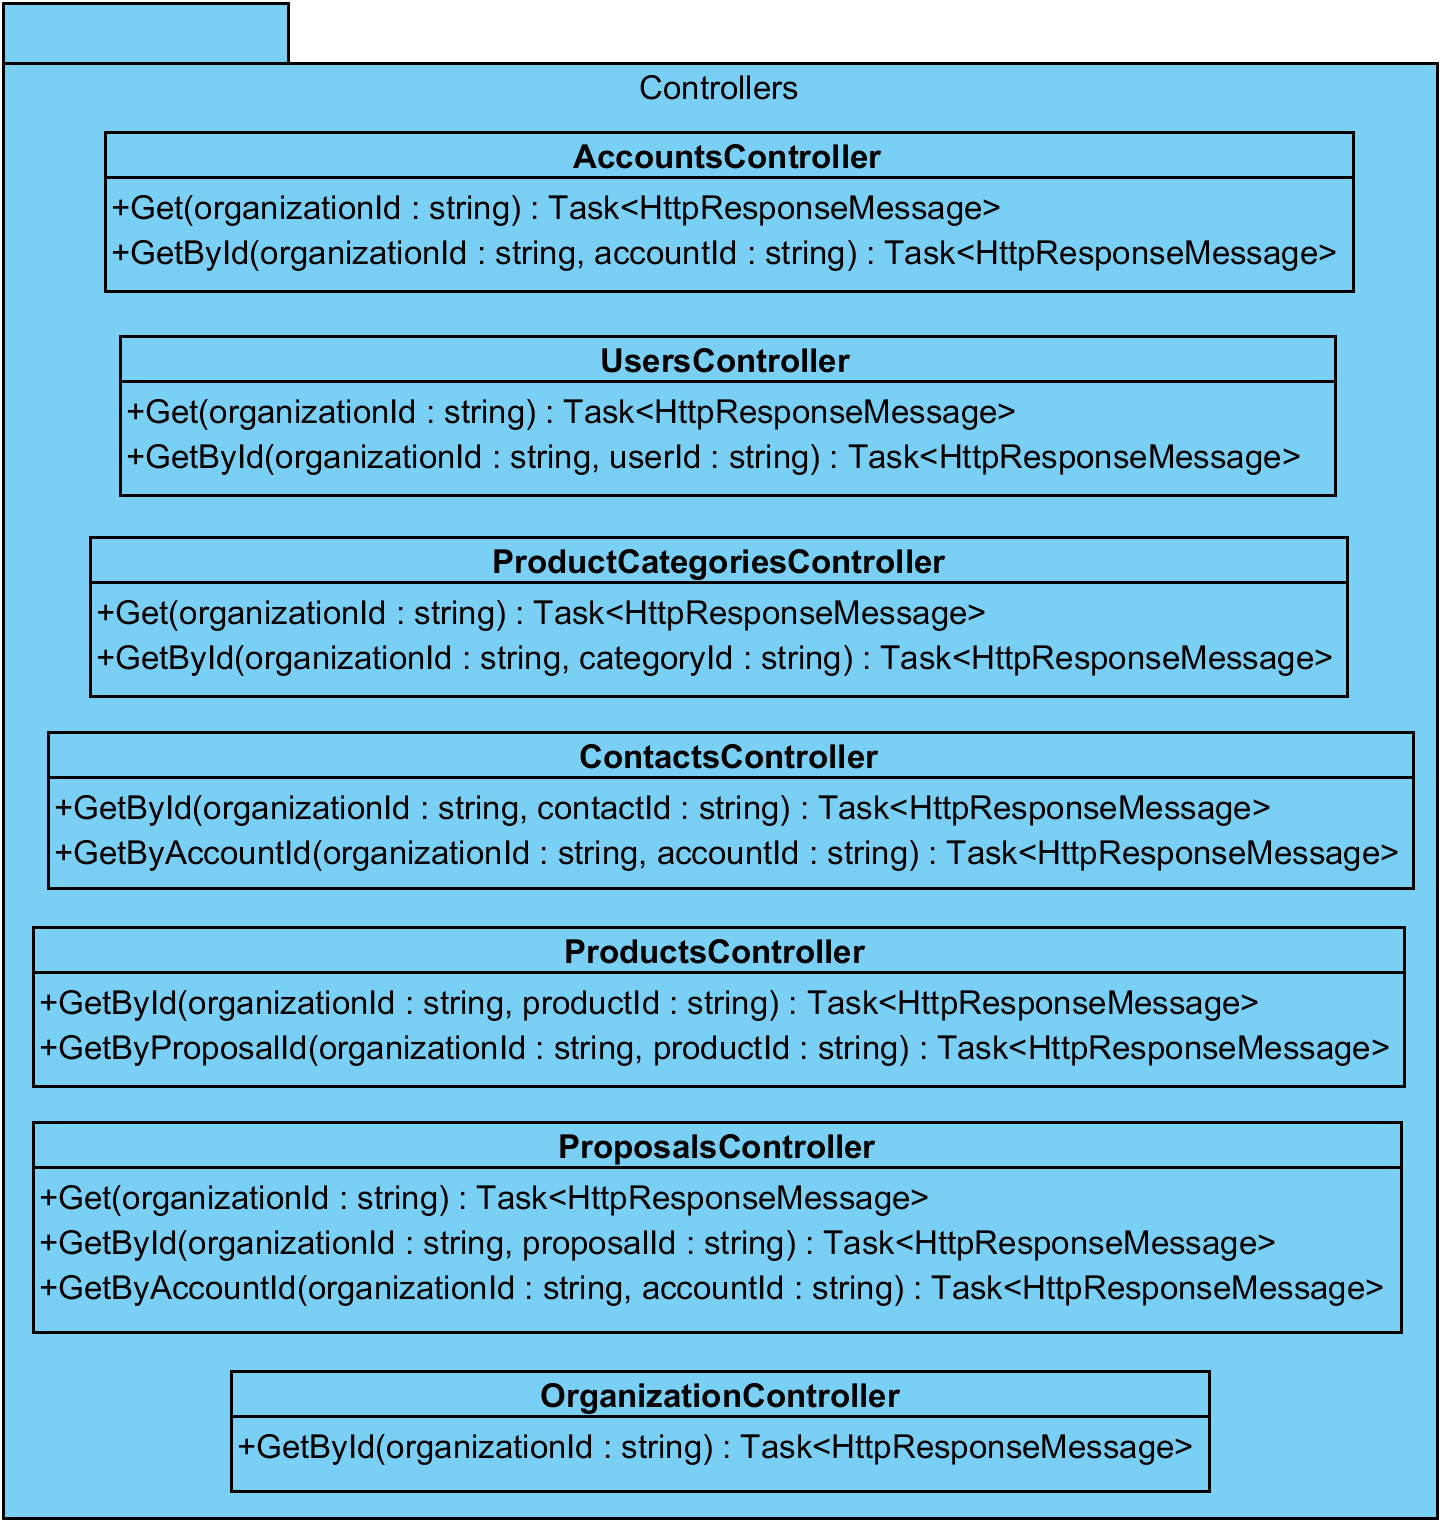
\includegraphics[width=\linewidth]{images/modules/Controllers}
	\caption{}
	\label{fig:controllers}
\end{figure}


Questo \glo{package} contiene tutte le classi controller contenenti i metodi necessari a rispondere alle richieste http effettuate alle \glo{route}.

\subsubsection{AccountsController (class)}

\paragraph{Descrizione:}
Classe che serve per gestire le chiamate http richiedenti dati relativi all'entità Account. Utilizzando la classe Athesys.ADCrm.Model::Crm (che implementa il design pattern Factory) vengono creati oggetti sui quali si possono invocare metodi per interrogare le API di uno specifico CRM.
I dati recuperati vengono incapsulati in una risposta http e ritornati ad ADProject.

\paragraph{Metodi:}\hfill
\begin{itemize}
	\itemsep0em 
	\item 
		\begin{lstlisting}
		Public async Task<HttpResponseMessage> Get(organizationId : string)
		\end{lstlisting}
		Metodo invocato quando viene inviata una richiesta http GET alla route "api/organization/{organizationId}/accounts", ritornado una risposta http contenente la lista di tutti gli Account censiti nel CRM.\\
		\textbf{\small Argomenti:}
		\begin{enumerate}[leftmargin=*]
			\itemsep0em 
			\item \begin{lstlisting}
			organizationId : string 
			\end{lstlisting}
			Rapprensenta l'identificativo univoco legato all'utenza aziendale con cui accedere al servizio CRM
		\end{enumerate}
		
	\item 
		\begin{lstlisting}
		Public async Task<HttpResponseMessage> GetById(organizationId : string, accountId : string)
		\end{lstlisting}
		Metodo invocato quando viene inviata una richiesta http GET alla route "api/organization/{organizationId}/accounts/{accountId}", ritornando una risposta http contenente l'Account avente id = {accountId}.\\
		\textbf{\small Argomenti:}
		\begin{enumerate}[leftmargin=*]
			\itemsep0em 
			\item 
				\begin{lstlisting}
				organizationId : string 
				\end{lstlisting}
				Rappresenta l'identificativo univoco legato all'utenza aziendale con cui accedere al servizio CRM
			\item 
				\begin{lstlisting}
				accountId : string
				\end{lstlisting}
				Rappresenta l'identificativo univoco legato ad un Account del CRM, attraverso il quale si andrà a richiedere i dati voluti
		\end{enumerate}
\end{itemize}

\subsubsection{ProposalsController (class)}

\paragraph{Descrizione:}
Classe che serve per gestire le chiamate http richiedenti dati relativi all'entità Proposal. Utilizzando la classe Athesys.ADCrm.Model::Crm (che implementa il design pattern Factory) vengono creati oggetti sui quali si possono invocare metodi per interrogare le API di uno specifico CRM. I dati recuperati vengono incapsulati in una risposta http e ritornati ad ADProject.

\paragraph{Metodi:}\hfill
\begin{itemize}
	\itemsep0em 
	\item 
	\begin{lstlisting}
	Public async Task<HttpResponseMessage> Get(organizationId : string)
	\end{lstlisting}
	Metodo invocato quando viene inviata una richiesta http GET alla route "api/organization/{organizationId}/proposals", ritornando una risposta http contenente tutte le offerte commerciali censite nel CRM.\\
	\textbf{\small Argomenti:}
	\begin{enumerate}[leftmargin=*]
		\itemsep0em 
		\item \begin{lstlisting}
		organizationId : string 
		\end{lstlisting}
		Rappresenta l'identificativo univoco legato all'utenza aziendale con cui accedere al servizio CRM.
	\end{enumerate}
	
	\item 
	\begin{lstlisting}
	Public async Task<HttpResponseMessage> GetById(organizationId : string,  proposalId : string)
	\end{lstlisting}
	Metodo invocato quando viene inviata una richiesta http GET alla route "api/organization/{organizationId}/proposals/{proposalId}", ritornando una risposta http contenente l'offerta commerciale avente id = {proposalId}.\\
	\textbf{\small Argomenti:}
	\begin{enumerate}[leftmargin=*]
		\itemsep0em 
		\item 
		\begin{lstlisting}
		organizationId : string 
		\end{lstlisting}
		Rapprensenta l'identificativo univoco legato all'utenza aziendale con cui accedere al servizio CRM;
		\item 
		\begin{lstlisting}
		proposalId : string
		\end{lstlisting}
		Rappresenta l'identificativo univoco legato ad un offerta commerciale del CRM, attraverso il quale si andrà a richiedere i dati voluti.
	\end{enumerate}

	\item 
	\begin{lstlisting}
	Public async Task<HttpResponseMessage> GetByAccountId(organizationId : string,  accountId : string)
	\end{lstlisting}
	Metodo invocato quando viene inviata una richiesta http GET alla route "api/organization/{organizationId}/accounts/{accountId}/proposals", ritornando una risposta http contenente la lista delle proposte legate all'account avente id = {proposalId}.\\
	\textbf{\small Argomenti:}
	\begin{enumerate}[leftmargin=*]
		\itemsep0em 
		\item 
		\begin{lstlisting}
		organizationId : string 
		\end{lstlisting}
		Rapprensenta l'identificativo univoco legato all'utenza aziendale con cui accedere al servizio CRM;
		\item 
		\begin{lstlisting}
		accountId : string
		\end{lstlisting}
		Rappresenta l'identificativo univoco legato all'account di un azienda cliente CRM, attraverso il quale si andrà a richiedere i dati voluti.
	\end{enumerate}
\end{itemize}



\vfill



\subsection{Athesys.ADCrm.Common}
\begin{sidewaysfigure}
	\begin{figure}[H]
		\centering
		\includegraphics[width=\linewidth]{images/modules/common}
		\caption{}
		\label{fig:common}
	\end{figure}
\end{sidewaysfigure}
Questo \glo{package} contiene il \glo{package} Data(avente le classi DTO) e tutte le interfacce che dovranno essere implementate diversamente per ogni CRM che si vuole collegare all'applicazione. 
%TODO: da modificare la descrizione

\subsubsection{IProposal (interface)}

\paragraph{Descrizione:}
Interfaccia che dovrà essere implementata dalle classi concrete Athesys.ADCrm.Salesforce::Proposal e\\ Athesys.ADCrm.Dynamics::Proposal, essa definisce i metodi utilizzati per interrogare i rispettivi CRM attraverso le API REST esposte, restituendo la risposta HTTP incapsulata all'interno di un DTO di tipo ResponseContainerData.

\paragraph{Metodi:}\hfill
\begin{itemize}
	\itemsep0em 
	\item 
	\begin{lstlisting}
	Task<ResponseContainerData<ProposalData>> GetAll()
	\end{lstlisting}
	Metodo da implementare per interrogare il CRM ritornando la lista di tutte le offerte commerciali censite nello stesso. Il metodo restituisce il DTO ResponseContainerData istanziato al tipo ProposalData essendo una classe \glo{generic}.\\
	
	\item 
	\begin{lstlisting}
	Task<ResponseContainerData<ProposalData>> GetById(proposalId : string)
	\end{lstlisting}
	Metodo da implementare per interrogare il CRM ritornando l'offerta commerciale avente id = {proposalId}. Il metodo restituisce il DTO ResponseContainerData istanziato al tipo ProposalData essendo una classe \glo{generic}.\\
	\textbf{\small Argomenti:}
	\begin{enumerate}[leftmargin=*]
		\itemsep0em 
		\item 
		\begin{lstlisting}
		proposalId : string
		\end{lstlisting}
		Rappresenta l'identificativo univoco legato ad un offerta commerciale del CRM, attraverso il quale si andrà a richiedere i dati voluti.
	\end{enumerate}
	
	\item 
	\begin{lstlisting}
	Task<ResponseContainerData<ProposalData>> GetByAccountId(accountId : string)
	\end{lstlisting}
	Metodo da implementare per interrogare il CRM ritornando la lista di tutte le offerte commerciali legate all'account avente id = {accountId}. Il metodo restituisce il DTO ResponseContainerData istanziato al tipo ProposalData essendo una classe \glo{generic}.\\
	\textbf{\small Argomenti:}
	\begin{enumerate}[leftmargin=*]
		\itemsep0em
		\item 
		\begin{lstlisting}
		accountId : string
		\end{lstlisting}
		Rappresenta l'identificativo univoco legato all'account di un azienda cliente CRM, attraverso il quale si andrà a richiedere i dati voluti.
	\end{enumerate}
\end{itemize}

\subsection{Athesys.ADCrm.API.Data}
Questo \glo{package} contiene tutti i vari DTO definiti per ogni entità di dati che si vuole restituire alle chiamate effettuate da ADProject ed inoltre quelle necessarie per gestire le risposte le risposte provenienti dai CRM. 
Segue in questa sezione una breve descrizione delle classi principali, sorvolando sui metodi delle stesse in quanto sono tutti \glo{accessors} \glo{getter} e \glo{setter}.
\begin{figure}[H]
	\centering
	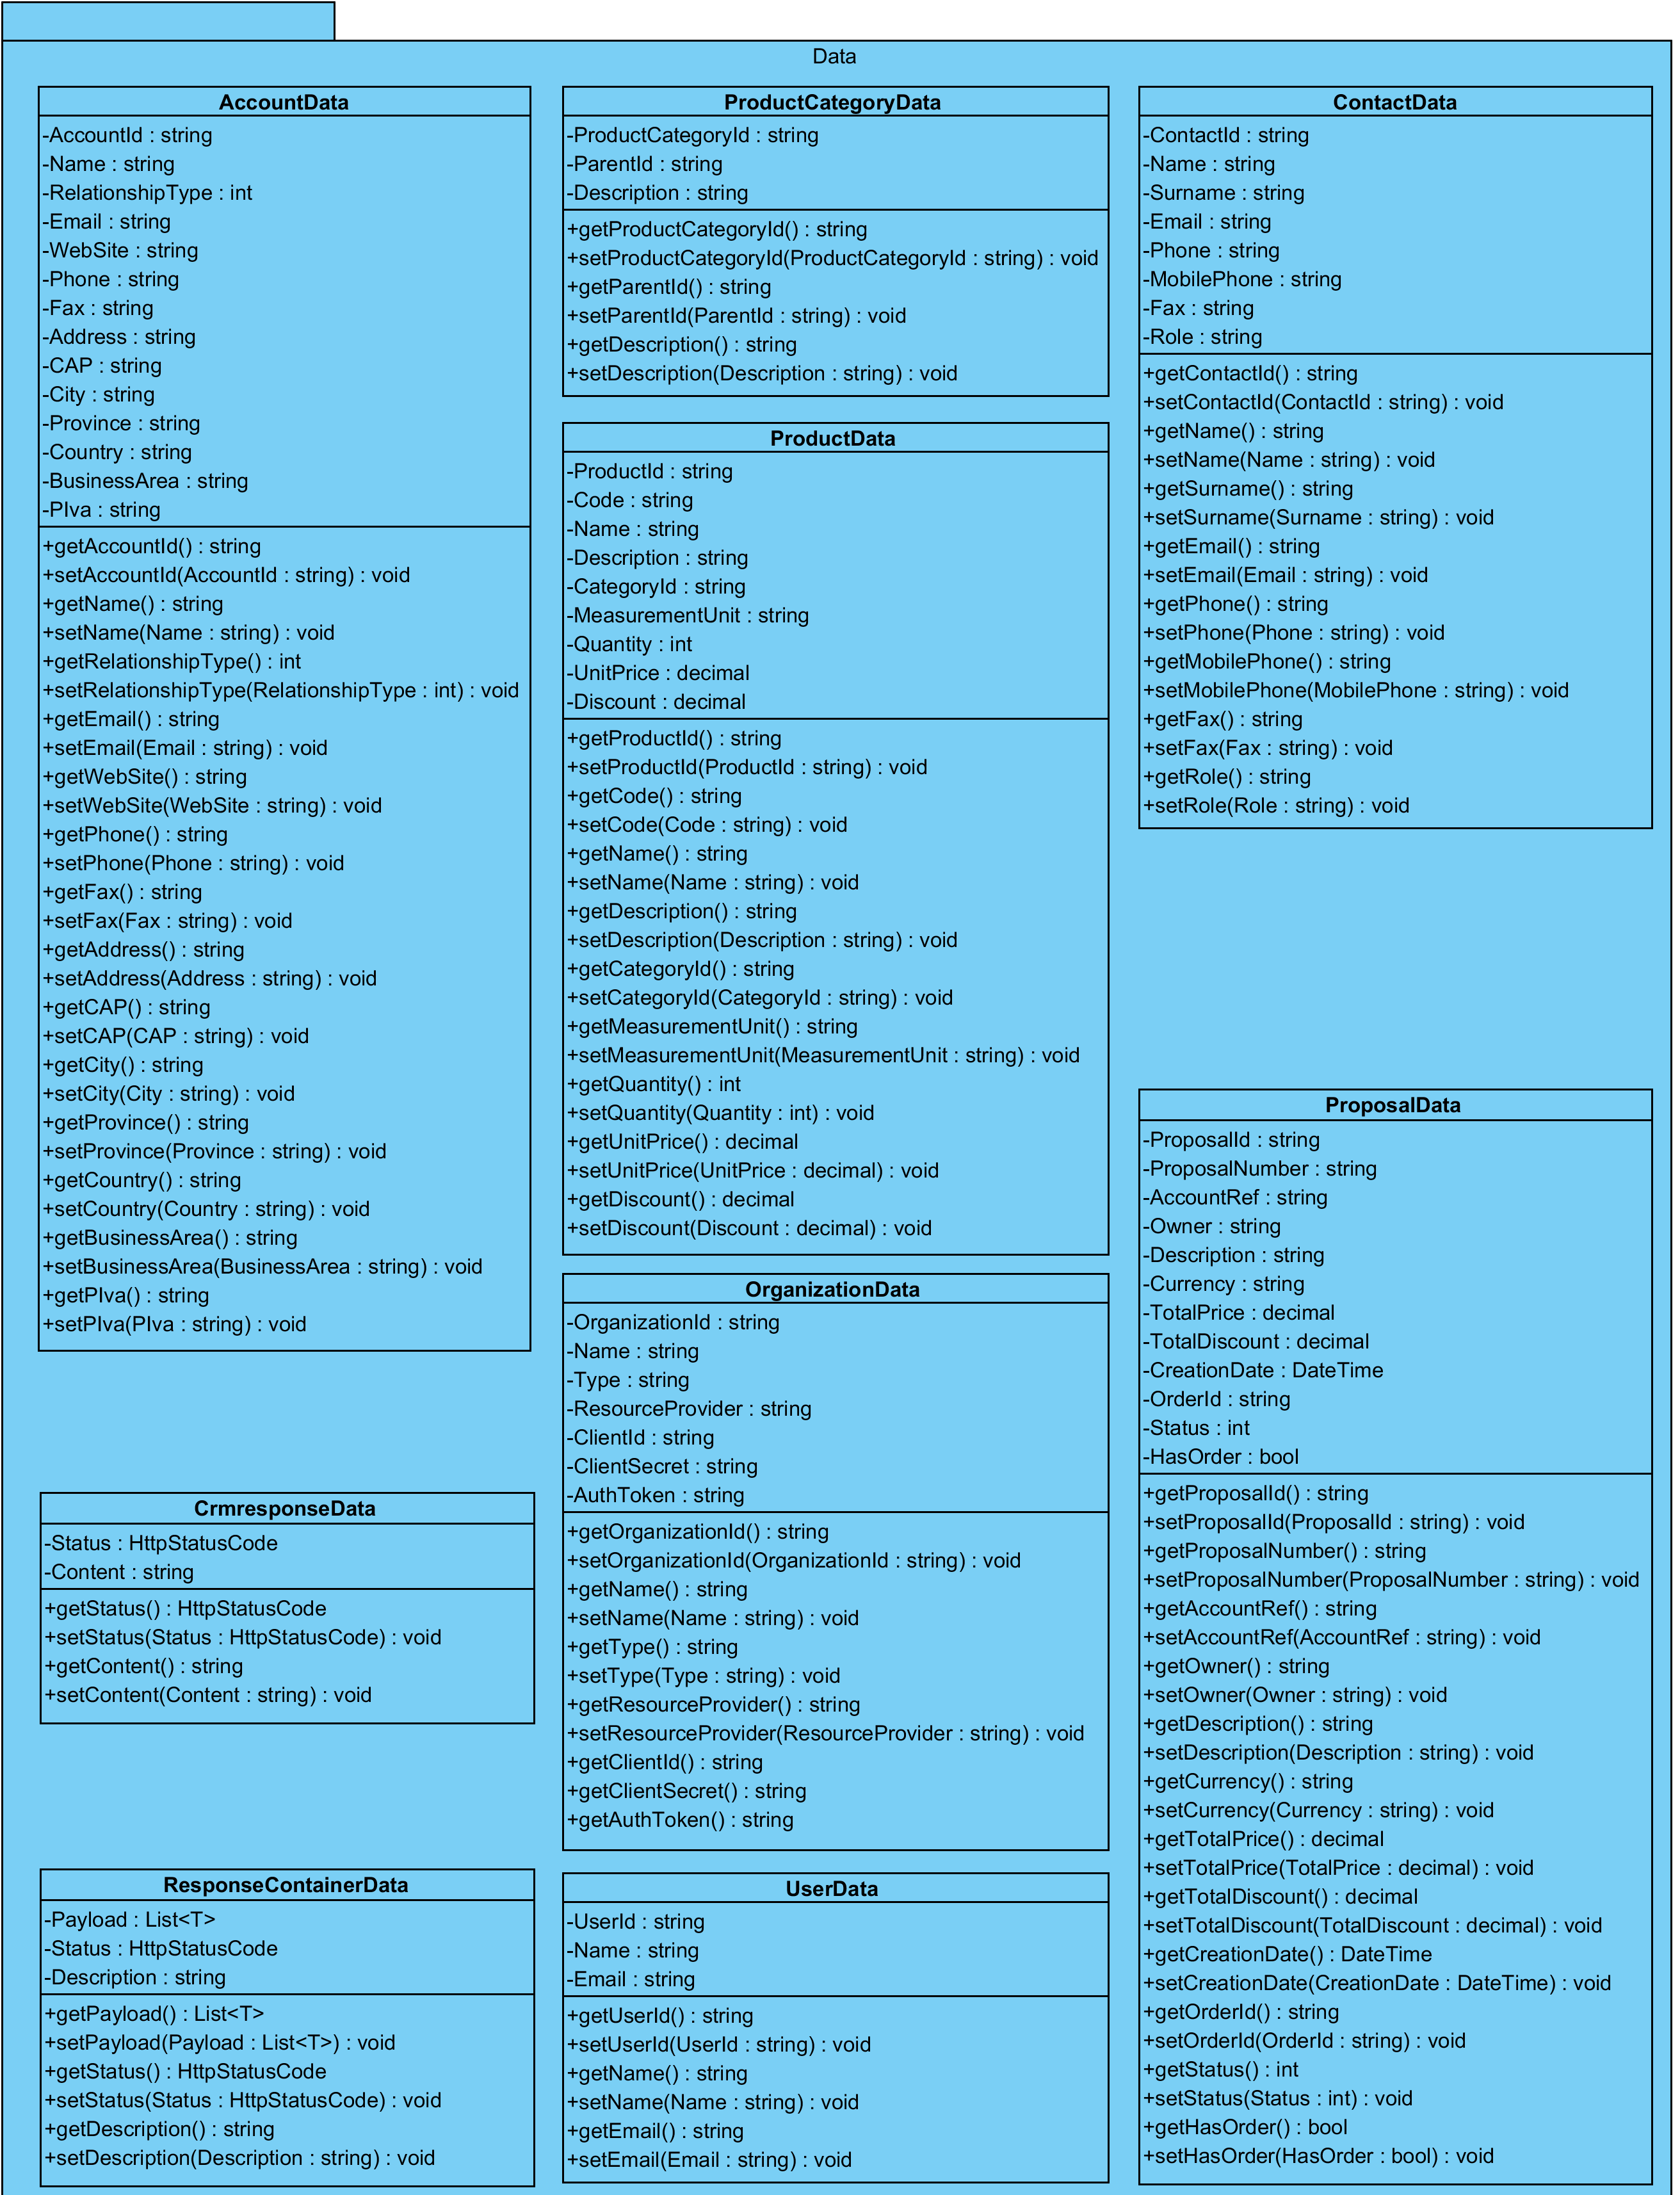
\includegraphics[width=\linewidth]{images/modules/Data}
	\caption{}
	\label{fig:data}
\end{figure}

\subsubsection{ProposalData (class)}
\paragraph{Descrizione:}
Classe che rappresenta un oggetto DTO per modellare l'entità \textit{Proposal}.
In essa sono presenti i metodi \glo{getter} e \glo{setter} e tutti i campi dati (privati) contenenti gli elementi che caratterizzano un offerta commerciale, quali: l'identificativo univoco della stessa, il cliente a cui è stata proposta, il costo totale, un eventuale sconto e molti altri dati.
Gli oggetti di questa classe, contenente i dati provenienti dal CRM, verranno incapsulati all'interno della risposta HTTP restituita ad ADProject.

\subsubsection{CrmResponseData (class)}
\paragraph{Descrizione:}
Classe che rappresenta un oggetto DTO per modellare le risposte HTTP provenienti dal CRM.
Questa classe ha solamente due campi dati (ed i relativi \glo{accessors}):
\begin{itemize}
	\item 	
	\begin{lstlisting}
	Private HttpStatusCode Status
	\end{lstlisting}
	In questo campo dati viene salvato il codice di stato HTTP della risposta mandata dal CRM;
	\item
	\begin{lstlisting}
	Private string Content
	\end{lstlisting}
	In questo campo dati viene salvato il \glo{Json} della risposta mandata dal CRM.
\end{itemize}

\subsubsection{ResponseContainerData (class)}
\paragraph{Descrizione:}
Classe che rappresenta un oggetto DTO per modellare le risposte HTTP da inviare a ADProject.
Questa classe ha tre campi dati (ed i relativi \glo{accessors}):
\begin{itemize}
	\item 	
	\begin{lstlisting}
	private List<T> Payload
	\end{lstlisting}
	In questo campo dati è una lista di \glo{generics} che viene istanziata al tipo di uno degli oggetti DTO di questo \glo{package} (AccountData,ProposalData,ProductData,ContactData,UserData,ProductCategoryData o OrganizationData);
	
	\item 	
	\begin{lstlisting}
	private HttpStatusCode Status
	\end{lstlisting}
	In questo campo dati viene salvato il codice di stato HTTP che dovrà assumere la risposta da inviare ad ADProject;
	
	\item
	\begin{lstlisting}
	private string Description
	\end{lstlisting}
	In questo campo dati, in caso di errore, viene aggiunta una breve descrizione testuale dello stesso.
\end{itemize}




\subsection{Athesys.ADCrm.Model}
Questo \glo{package} contiene tutte le classi concrete in comune tra i CRM che si vogliono collegare all'applicazione.
La classe principale del \glo{package} è Athesys.ADCrm.Model::Crm.
\subsubsection{Crm (class)}
\paragraph{Descrizione:}
Questa classe implementa il design pattern Factory ed è usata dai controllers per produrre oggetti concreti di un particolare CRM (su cui invocare i metodi per recuperare i dati dallo stesso) senza conoscere a priori il tipo di CRM richiesto (Dynamics o SalesForce).

\begin{figure}[H]
	\centering
	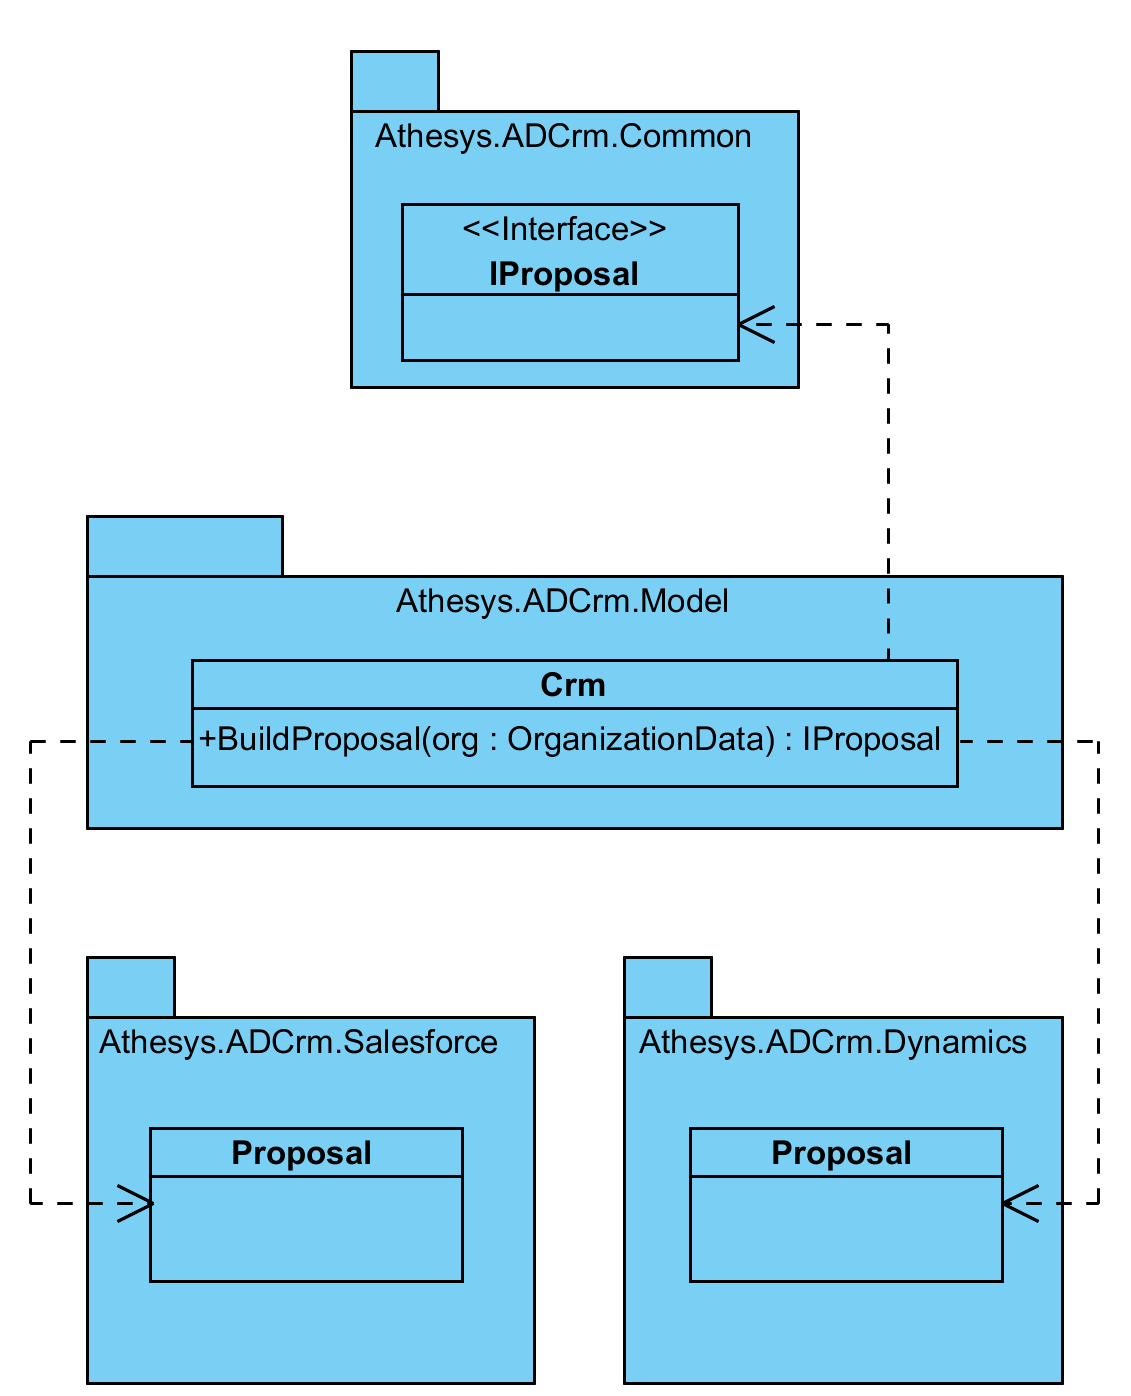
\includegraphics[width=\linewidth]{images/factoryInADCrm}
	\caption{Diagramma semplificato del pattern Factory per ADCrm}
	\label{fig:factoryInADCrm}
\end{figure}
Di seguito vengono riportati alcuni metodi significativi della classe per esemplificarne il funzionamento generale.


\paragraph{Metodi:}\hfill
\begin{itemize}
	\itemsep0em 
	\item 
	\begin{lstlisting}
	  public static async Task<OrganizationData> BuildOrganization(string organizationId)	
	\end{lstlisting}
	Metodo che costruisce un oggetto di tipo OrganizationData, appartenente ad un particolare CRM, in base alla tipologia del parametro passato.
	Tutti i campi dati dell'oggetto ritornato vengono impostati dal database dell'applicazione che contiene i parametri di connessione ai vari CRM.
	\\
	\textbf{\small Argomenti:}
	\begin{enumerate}[leftmargin=*]
		\itemsep0em 
		\item 
		\begin{lstlisting}
		organizationId : string
		\end{lstlisting}
		Rappresenta la tipologia di CRM a cui ci si deve collegare. Questo dati si ottiene grazie alle route definite nella sezione \ref{apiRest} (eg. api/organization/\{\textbf{organizationId}\}/accounts).
	\end{enumerate}
	
	\item 
	\begin{lstlisting}
     public static IProposal BuildProposal(OrganizationData org)
	\end{lstlisting}
	Metodo che, in base alla tipologia di organizzazione passata per parametro, costruisce un oggetto Proposal per un particolare tipo di CRM\\
	\textbf{\small Argomenti:}
	\begin{enumerate}[leftmargin=*]
		\itemsep0em
		\item 
		\begin{lstlisting}
		org : OrganizationData
		\end{lstlisting}
		Rappresenta la tipologia di CRM da cui si vogliono recuperare le proposte commerciali.
	\end{enumerate}
\end{itemize}
 
\subsection{Athesys.ADCrm.Salesforce}
Questo \glo{package} contiene tutte le classi che implementano le interfacce definite in Athesys.ADCrm.Common e, sviluppando  restituiscono ai controllers di Athesys.ADCrm.API i vari oggetti DTO delle entità del \glo{package} Athesys.ADCrm.Common.Data.
Di seguito vengono descritte brevemente le uniche tre classi che hanno un comportamento diverso da quanto sopracitato.

\subsubsection{IdentityProvider (class)}
\paragraph{Descrizione:}
%TODO
\subsubsection{ResponceMapper (class)}
\paragraph{Descrizione:}
%TODO
\subsubsection{Entity (class)}
\paragraph{Descrizione:}
%TODO

\subsection{Athesys.ADCrm.Dynamics}
Questo \glo{package} contiene tutte le classi che implementano le interfacce definite in Athesys.ADCrm.Common e restituiscono ai controller di Athesys.ADCrm.API i vari oggetti DTO di tipo Athesys.ADCrm.Common.Data al fine di incapsularli nella risposta HTTP.